\subsection{ID regression}
\label{sec:result_ID_regression}
The parameters within the two models have been identified with Inverse dynamics (ID) regression on a set of manoeuvring model tests conducted with a scale model of the WPCC. The model tests (see \autoref{fig:model_tests}) consist of zigzag10/10, and zigzag20/20 tests to port and starboard as well as some yaw rate tests and self propulsion test on a straight course. All of the test are used in the training dataset to identify the parameters within the Abkowitz and Semi-empirical models.
\begin{figure}[h!]
    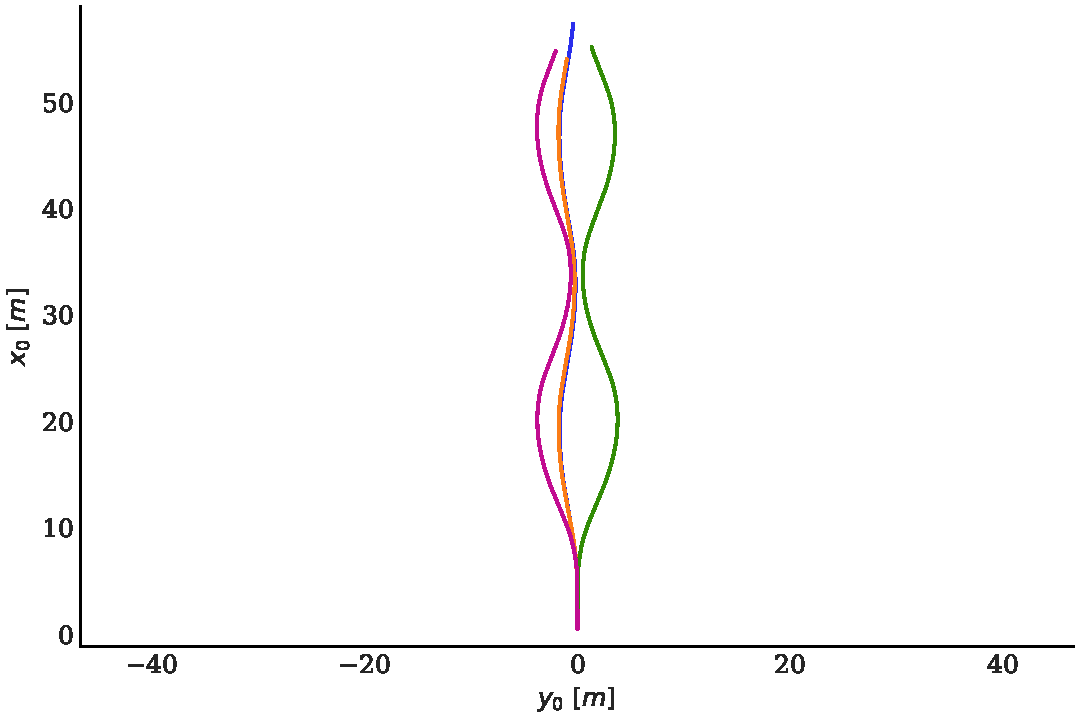
\includegraphics[width=\textwidth]{figures/result_ID_regression.model_tests.pdf}
    \caption{Model tests trajectories.}
    \label{fig:model_tests}
\end{figure}
\autoref{fig:ID_regression_ID_N} shows predicted yawing moments for one of the zigzag20/20 tests predicted with the two models identified by inverse dynamics and also predicted by the Semi-empirical model identified with VCT regression. The yawing moment from the zigzag experiment, estimated with inverse dynamics, has also been added to these graphs -- as a reference. It seems that the the yawing moments are similar for all models and the experimental data. It can also be seen that the Semi-empirical model VCT and ID predicts the exact same rudder yawing moment $N_R$, since they both use the same deterministic semi-empirical rudder model -- the yawing moments from the hull $N_H$ are therefore similar for these models. The rudder yawing moment from the Abkowitz model ID is however very different, so that the yawing moments from the hull $N_H$ are also very different. This means that the total yawing moment is the same for all models, but the decomposition to hull and rudder moments turns out to be very different.
%\begin{figure}[h!]
%    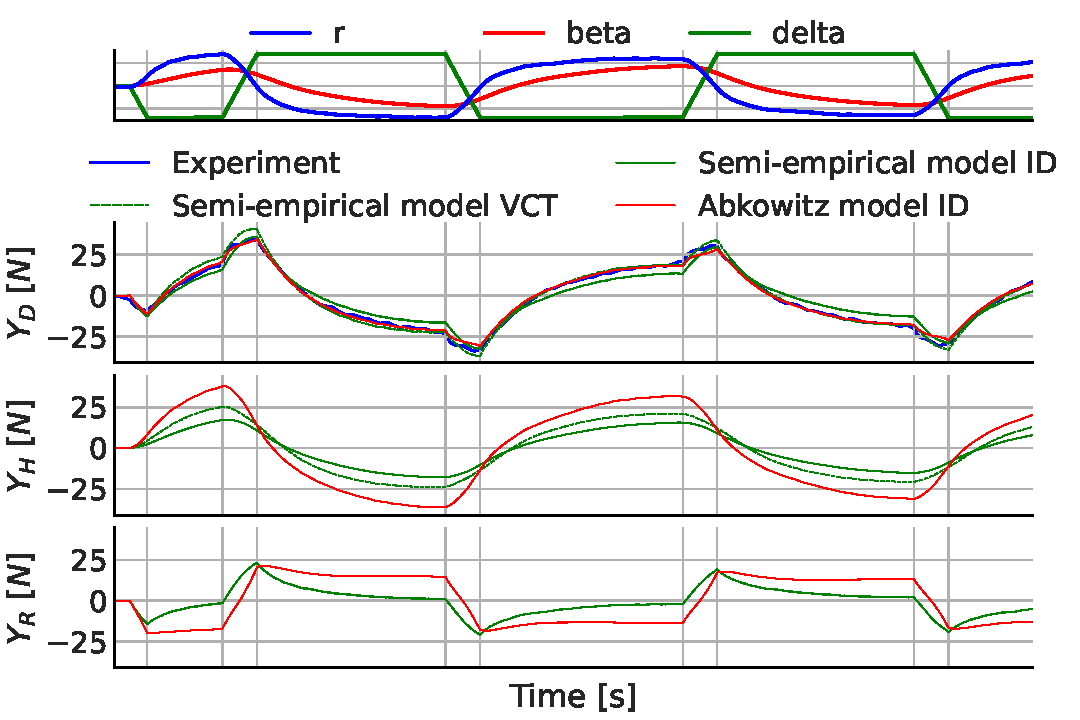
\includegraphics[width=\textwidth]{figures/result_ID_regression.ID_regression_ID_Y.pdf}
%    \caption{}
%    \label{fig:ID_regression_ID_Y}
%\end{figure}
\begin{figure}[h!]
    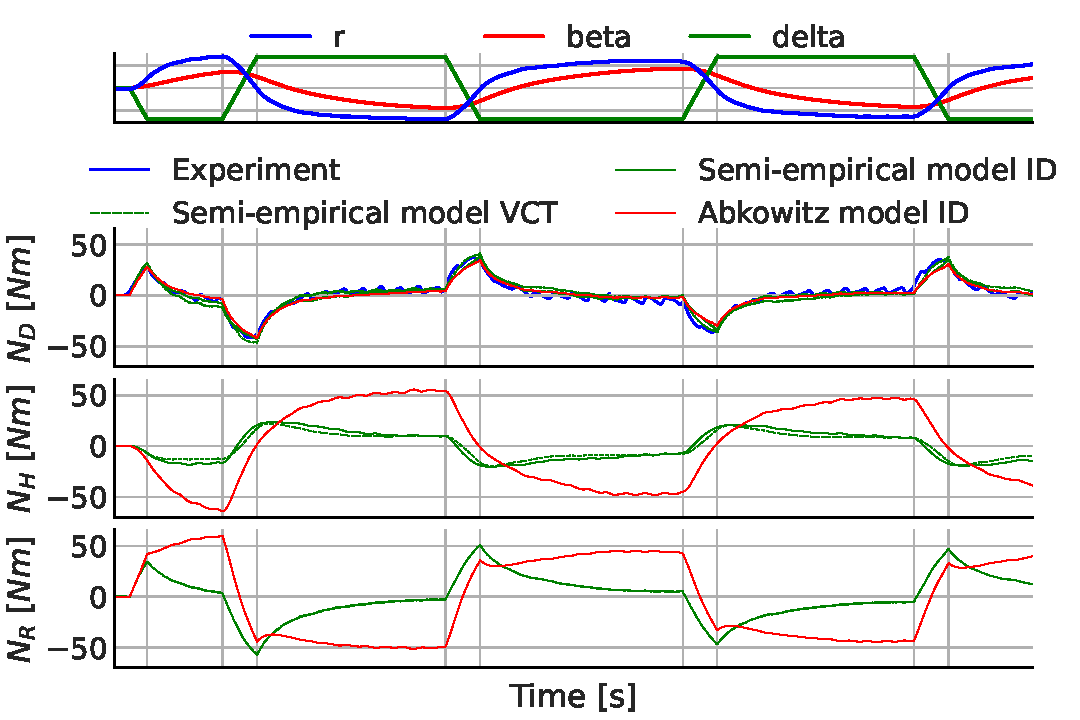
\includegraphics[width=\textwidth]{figures/result_ID_regression.ID_regression_ID_N.pdf}
    \caption{Comparison of the total yawing moment acting on the ship: predicted with the Semi-empirical VCT model, predicted with the Semi-empirical ID model, predicted with the Abkowitz ID model, and the corresponding values from a zigzag20/20 test estimated with inverse dynamics.}
    \label{fig:ID_regression_ID_N}
\end{figure}

\begin{figure}[h!]
    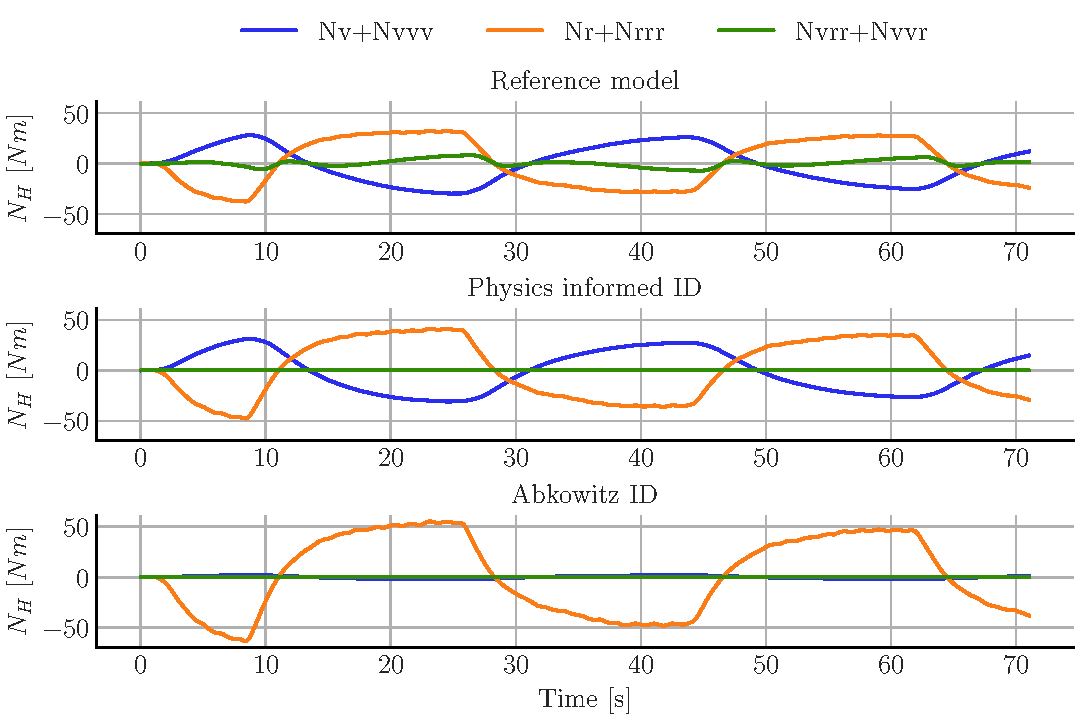
\includegraphics[width=\textwidth]{figures/result_ID_regression.ID_regression_N_decomposition.pdf}
    \caption{}
    \label{fig:ID_regression_N_decomposition}
\end{figure}